\section{Introduction}\label{sec:introduction}

\looseness=-1
Self-Consistency (SC) \citep{wang2023sc} selects the majority answer across $K$ chain-of-thought traces, a strategy grounded in the Condorcet Jury Theorem: independent voters converge to truth \citep{condorcet1785, ladha1992correlated}. In practice, SC's gains plateau for strong models \citep{loo2025reevaluating, byerly2025selfconsistency}, and correlated LLM errors \citep{kim2025correlated} reduce the effective ensemble size \citep{dietterich2000ensemble}. A natural remedy is to move beyond simple vote-counting: extract logical constraints from the traces, as in neuro-symbolic approaches \citep{pan2023logiclm, olausson2023linc, ye2024satlm}, and let a provably sound solver adjudicate. If the solver can filter contradictions and enforce logical consistency, it should recover information that raw majority voting discards.

\begin{figure*}[t!]
\centering
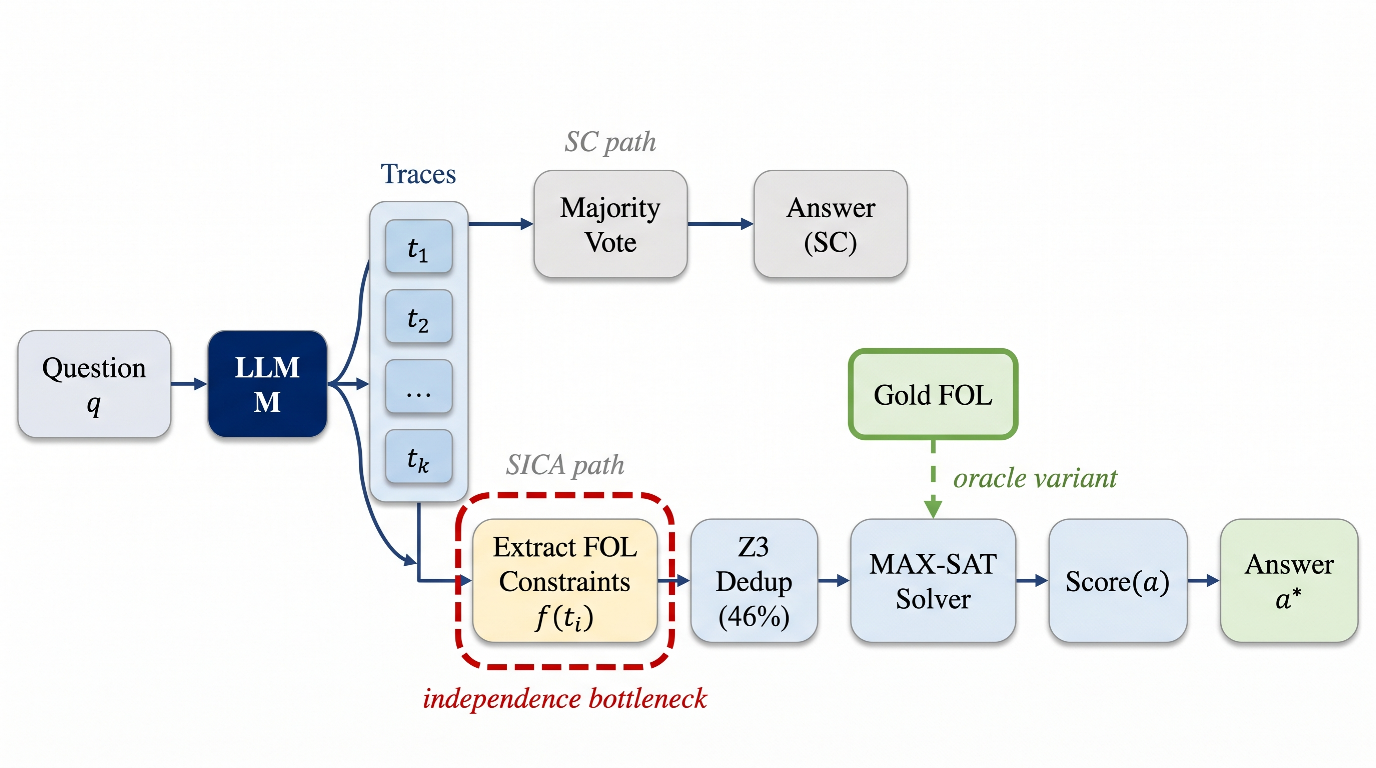
\includegraphics[width=0.88\textwidth]{figures/fig1_pipeline_v11.pdf}
\caption{The SICA pipeline. SC selects the majority answer from $K$ traces. SICA extracts logical constraints, deduplicates, and solves MAX-SAT via Z3. Red dashed box: the independence bottleneck. Dashed arrow: oracle variant with gold FOL.}
\label{fig:pipeline}
\end{figure*}

\looseness=-1
We test this intuition through Symbolic Invariant Consensus Aggregation (SICA), which extracts logical constraints from reasoning traces, deduplicates them, and selects answers via weighted partial MAX-SAT (\S\ref{sec:pipeline}; Figure~\ref{fig:pipeline}). Across six models (7B--32B), four benchmarks, and multi-seed replication, SICA produces answers identical to majority voting on most problems; no condition shows a significant positive effect after correction for multiple comparisons (Table~\ref{tab:main_results}). The failure lies not in the solver but in the constraints it operates on: self-extracted constraints systematically support the model's majority answer, a robust empirical regularity we term \emph{symbolic confirmation bias} (\S\ref{sec:confirmation-bias}), distinct from trace-level unfaithfulness \citep{turpin2023language, wan2025unveiling}. Because each trace determines both an answer and its constraints, the formal verification channel approximately reduces to a weighted echo of the majority vote under the degeneration condition (Observation~1).

\looseness=-1
This bias is not confined to a single model or task. Symbolic confirmation bias holds across nine models from 7B to frontier scale, and 27 training-free remediation strategies spanning four categories (prompt diversity, constraint filtering, multi-agent debate, and cross-model extraction) all produce neutral-to-negative results (\S\ref{sec:remediation}). A persistent independence--accuracy trade-off emerges: methods that break trace correlation (e.g., multi-agent debate; \citealp{liang2023encouraging, du2023improving}) destroy accuracy, while methods that preserve accuracy fail to achieve independence. Prior work demonstrates that LLMs cannot self-correct reasoning without external feedback \citep{huang2024selfcorrect, kamoi2024selfcorrect}; our analysis provides a concrete mechanism for these findings via the $M{\to}T{\to}(A,C)$ generation structure---where a model $M$ generates traces $T$ that determine both answers $A$ and constraints $C$---so constraints are downstream of the same generative process that produces the answers they are meant to check.

\looseness=-1
The bottleneck lies in self-extraction itself, not in solver capability or model scale. Cross-architecture verification escapes this bottleneck: a structurally independent verifier yields significant gains when it exceeds the generator's accuracy, with benefit governed by a capability-gap pattern between verifier and generator (\S\ref{sec:cross-arch}). This parallels test-time compute scaling \citep{snell2025scaling}, where additional inference budget faces diminishing returns once effective ensemble diversity saturates. Three lightweight diagnostics derived from a pilot run enable practitioners to predict a priori whether a self-extraction-based aggregation method will improve over SC (\S\ref{sec:diagnostic-framework}).

Our contributions are:
\begin{enumerate}[nosep,leftmargin=*]
\item \textbf{The symbolic mirage.} Provably sound Z3 verification becomes vacuous under self-extraction. We diagnose the underlying mechanism: self-extracted constraints inherit the generating model's distributional prior (symbolic confirmation bias), reducing SICA to majority vote under source-attribution scoring (Observation~1). The pattern holds across nine models and 27 training-free variants (\S\ref{sec:confirmation-bias}, \S\ref{sec:remediation}).

\item \textbf{Diagnostic framework.} Three lightweight diagnostics characterize failure modes across all tested conditions within the self-extraction paradigm, with prospective validation on held-out model families; these give practitioners a priori failure-mode diagnosis from a pilot run (\S\ref{sec:diagnostic-framework}).

\item \textbf{Cross-architecture escape.} Structurally independent verification breaks the bottleneck: a cross-architecture verifier restores corrective signal, with gain governed by a capability-gap pattern between verifier and generator (\S\ref{sec:cross-arch}).
\end{enumerate}

